% Options for packages loaded elsewhere
\PassOptionsToPackage{unicode}{hyperref}
\PassOptionsToPackage{hyphens}{url}
%
\documentclass[
]{article}
\usepackage{amsmath,amssymb}
\usepackage{iftex}
\ifPDFTeX
  \usepackage[T1]{fontenc}
  \usepackage[utf8]{inputenc}
  \usepackage{textcomp} % provide euro and other symbols
\else % if luatex or xetex
  \usepackage{unicode-math} % this also loads fontspec
  \defaultfontfeatures{Scale=MatchLowercase}
  \defaultfontfeatures[\rmfamily]{Ligatures=TeX,Scale=1}
\fi
\usepackage{lmodern}
\ifPDFTeX\else
  % xetex/luatex font selection
\fi
% Use upquote if available, for straight quotes in verbatim environments
\IfFileExists{upquote.sty}{\usepackage{upquote}}{}
\IfFileExists{microtype.sty}{% use microtype if available
  \usepackage[]{microtype}
  \UseMicrotypeSet[protrusion]{basicmath} % disable protrusion for tt fonts
}{}
\makeatletter
\@ifundefined{KOMAClassName}{% if non-KOMA class
  \IfFileExists{parskip.sty}{%
    \usepackage{parskip}
  }{% else
    \setlength{\parindent}{0pt}
    \setlength{\parskip}{6pt plus 2pt minus 1pt}}
}{% if KOMA class
  \KOMAoptions{parskip=half}}
\makeatother
\usepackage{xcolor}
\usepackage[margin=1in]{geometry}
\usepackage{graphicx}
\makeatletter
\def\maxwidth{\ifdim\Gin@nat@width>\linewidth\linewidth\else\Gin@nat@width\fi}
\def\maxheight{\ifdim\Gin@nat@height>\textheight\textheight\else\Gin@nat@height\fi}
\makeatother
% Scale images if necessary, so that they will not overflow the page
% margins by default, and it is still possible to overwrite the defaults
% using explicit options in \includegraphics[width, height, ...]{}
\setkeys{Gin}{width=\maxwidth,height=\maxheight,keepaspectratio}
% Set default figure placement to htbp
\makeatletter
\def\fps@figure{htbp}
\makeatother
\setlength{\emergencystretch}{3em} % prevent overfull lines
\providecommand{\tightlist}{%
  \setlength{\itemsep}{0pt}\setlength{\parskip}{0pt}}
\setcounter{secnumdepth}{-\maxdimen} % remove section numbering
\usepackage{eso-pic,graphicx,transparent}
\usepackage{booktabs}
\usepackage{longtable}
\usepackage{array}
\usepackage{multirow}
\usepackage{wrapfig}
\usepackage{float}
\usepackage{colortbl}
\usepackage{pdflscape}
\usepackage{tabu}
\usepackage{threeparttable}
\usepackage{threeparttablex}
\usepackage[normalem]{ulem}
\usepackage{makecell}
\usepackage{xcolor}
\ifLuaTeX
  \usepackage{selnolig}  % disable illegal ligatures
\fi
\usepackage{bookmark}
\IfFileExists{xurl.sty}{\usepackage{xurl}}{} % add URL line breaks if available
\urlstyle{same}
\hypersetup{
  pdftitle={Displacement and Solutions Dynamics},
  pdfauthor={DTM - Data for Solution},
  hidelinks,
  pdfcreator={LaTeX via pandoc}}

\title{Displacement and Solutions Dynamics}
\usepackage{etoolbox}
\makeatletter
\providecommand{\subtitle}[1]{% add subtitle to \maketitle
  \apptocmd{\@title}{\par {\large #1 \par}}{}{}
}
\makeatother
\subtitle{Linked to Displacement Drivers}
\author{DTM - Data for Solution}
\date{2024-10-20}

\begin{document}
\maketitle

\AddToShipoutPictureFG{
\AtPageCenter{% or \AtTextCenter
\makebox[0pt]{\rotatebox[origin=c]{45}{%
\scalebox{10}{\texttransparent{0.1}{DRAFT}}%
}}
}
}

\section{Climate IDP vs Intention}\label{climate-idp-vs-intention}

In some countries, internally displaced persons (IDPs) who have been
displaced due to conflict are more likely to express an intention to
return home once the conflict subsides. In contrast, climate-displaced
IDPs may be more inclined to seek local integration, recognizing that
the climate is unlikely to improve and that urban integration offers a
more sustainable future. This document will examine this hypothesis in
the context of Somalia, using data from the Durable Solution Progress
(DSP) survey.

In the DSP survey, respondents were asked, ``What was the primary reason
for leaving your place of origin?'' This question was used to classify
households based on whether they were displaced due to climate-related
shocks, conflict, or other reasons. The choices and classifications are
outlined below:

\begin{table}[h]
\centering
\caption{\label{tab:unnamed-chunk-1}Choice classification}
\centering
\begin{tabular}[t]{>{}l|l}
\hline
Classification & Choices\\
\hline
 & Drought/lack of rain\\
\cline{2-2}
\multirow{-2}{*}[0.5\dimexpr\aboverulesep+\belowrulesep+\cmidrulewidth]{\raggedright\arraybackslash \textbf{Climate change related displacement}} & Flooding/excessive rain\\
\cline{1-2}
 & Conflict/security situation\\
\cline{2-2}
 & Eviction (from land)\\
\cline{2-2}
 & Eviction (from house)\\
\cline{2-2}
\multirow{-4}{*}[1.5\dimexpr\aboverulesep+\belowrulesep+\cmidrulewidth]{\raggedright\arraybackslash \textbf{Conflict related displacement}} & Fear of persecution\\
\cline{1-2}
 & Poor economic conditions\\
\cline{2-2}
\multirow{-2}{*}[0.5\dimexpr\aboverulesep+\belowrulesep+\cmidrulewidth]{\raggedright\arraybackslash \textbf{Livelihood related displacement}} & Not able to pay rent\\
\cline{1-2}
 & Lack of basic services\\
\cline{2-2}
\multirow{-2}{*}[0.5\dimexpr\aboverulesep+\belowrulesep+\cmidrulewidth]{\raggedright\arraybackslash \textbf{Service facility related displacement}} & Lack of shelter\\
\cline{1-2}
 & Discrimination by the community\\
\cline{2-2}
\multirow{-2}{*}[0.5\dimexpr\aboverulesep+\belowrulesep+\cmidrulewidth]{\raggedright\arraybackslash \textbf{NOT COSIDERED}} & Others\\
\hline
\end{tabular}
\end{table}

\subsection{Displacement reason}\label{displacement-reason}

The majority of IDPs reported being displaced primarily due to
climate-related issues, followed by conflict-related reasons. The chart
below illustrates the overall percentage distribution of the various
causes of displacement.

\begin{figure}[H]

{\centering 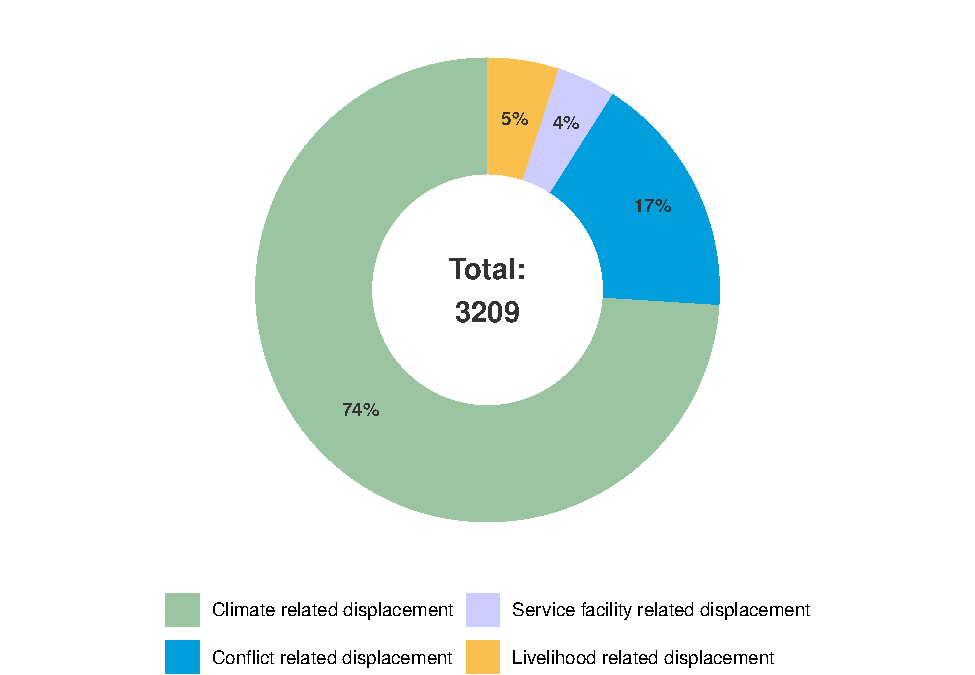
\includegraphics[width=0.7\linewidth,height=0.7\textheight]{climate_vs_conflict_files/figure-latex/dis_type-1} 

}

\caption{Reason of Displacement}\label{fig:dis_type}
\end{figure}

A similar trend is observed across each city, though there are
noticeable differences in the percentages. For instance, in
\emph{Bardaale}, \textbf{\emph{93\%}} of households reported that
climate shocks were the primary reason for displacement, while in
\emph{Xudur} and \emph{Doolow}, the figures are \textbf{\emph{60\%}} and
\textbf{\emph{65\%}}, respectively. Conversely, in \emph{Kismayo} and
\emph{Xudur}, the proportion of conflict-induced IDPs is relatively
higher compared to other cities. The charts below display the reasons
for displacement by city.

\begin{figure}[H]

{\centering 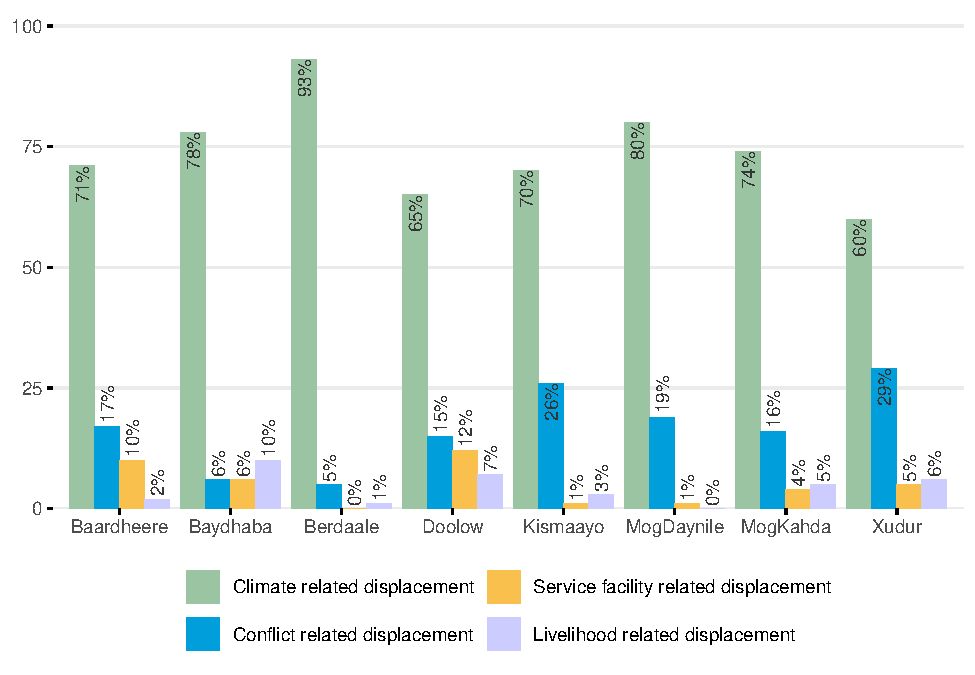
\includegraphics[width=0.7\linewidth,height=0.7\textheight]{climate_vs_conflict_files/figure-latex/dis_type_city-1} 

}

\caption{Reason of Displacement by City}\label{fig:dis_type_city}
\end{figure}

\subsubsection{Relationship between IDP classification and Intention to
return place of
origin}\label{relationship-between-idp-classification-and-intention-to-return-place-of-origin}

The graph below shows the percentage of IDP households reporting their
intention to remain in various locations by displacement type. Among
those who were originally displaced due to conflict,a significant number
of people want to return to their place of origin(\textbf{\emph{46\%}}).
In contrast, of those displaced by climate-related issues, only
\textbf{\emph{34\%}} intended to retunr place of origin.

\begin{figure}[H]

{\centering 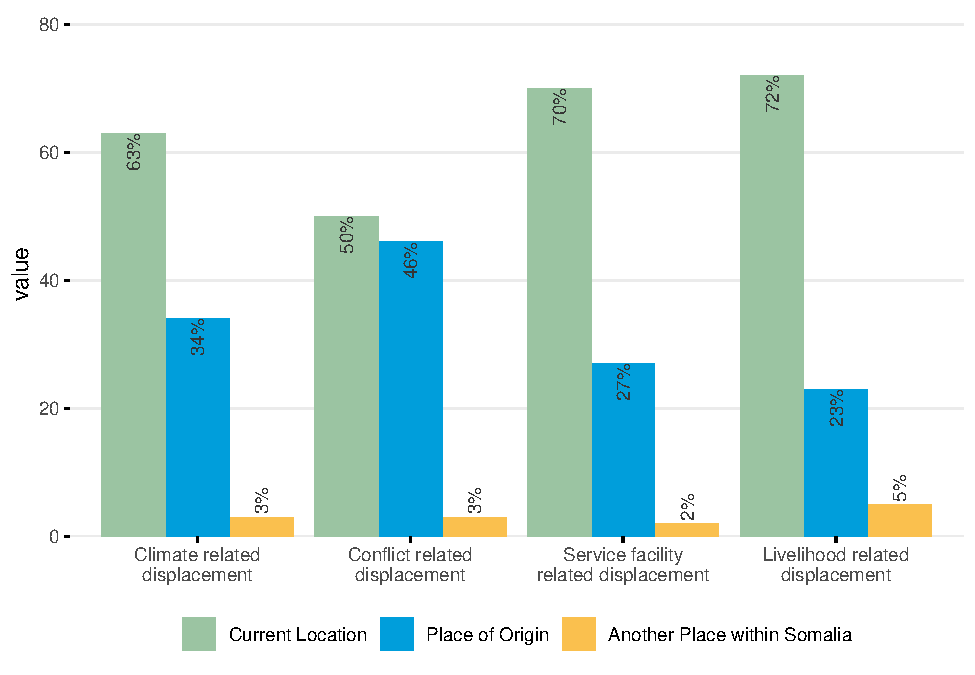
\includegraphics[width=0.8\linewidth,height=0.8\textheight]{climate_vs_conflict_files/figure-latex/idp_int_class-1} 

}

\caption{IDP intention vs classification}\label{fig:idp_int_class}
\end{figure}

\textbf{City-level} analysis also shows similar results \emph{(figure
\textbf{\textcolor{blue}{\ref{fig:in_classi_city}}})} . For instance, in
Berdale, \textbf{\emph{73\%}} of IDP households displaced by conflict
expressed an intention to return to their place of origin. However,
different trends were observed in some cities, such as Kismayo and
Mogadishu Daynile, where the patterns deviate \footnote{\textbf{WHY?}}.

\subsubsection{Singificance test}\label{singificance-test}

The overall data \emph{(figure
\textbf{\textcolor{blue}{\ref{fig:idp_int_class}}})} indicates a higher
tendency for IDPs to return to their place of origin if they were
initially displaced due to conflict-related issues. To further examine
this hypothesis, a Chi-square test\footnote{The Chi-square test is a
  statistical method used to assess whether there is a significant
  association between two categorical variables. A small p-value
  (typically \textless{} 0.05) indicates a statistically significant
  relationship between the variables.} was conducted..

\begin{itemize}
\item
  \textbf{\emph{Null Hypothesis:}} There is no significant relationship
  between IDP classification (reason for displacement) and the intention
  to return to their place of origin.
\item
  \textbf{\emph{Alternative Hypothesis:}} IDPs who left their place of
  origin due to conflict are more likely to intend to return once the
  conflict has ended.
\end{itemize}

\subsubsection{Result}\label{result}

\begin{verbatim}
##            Chisq               df          p.value 
## 51.1969080939965 12.0000000000000  0.0000008598522
\end{verbatim}

\textbf{Interpretation:} Given that the p-value is extremely small, well
below the conventional significance threshold of \emph{0.05}, we can
reject the null hypothesis. This suggests that it is highly unlikely the
result occurred by chance, indicating a meaningful relationship between
the reason for displacement and the preferred location to stay.

\begin{figure}[H]

{\centering 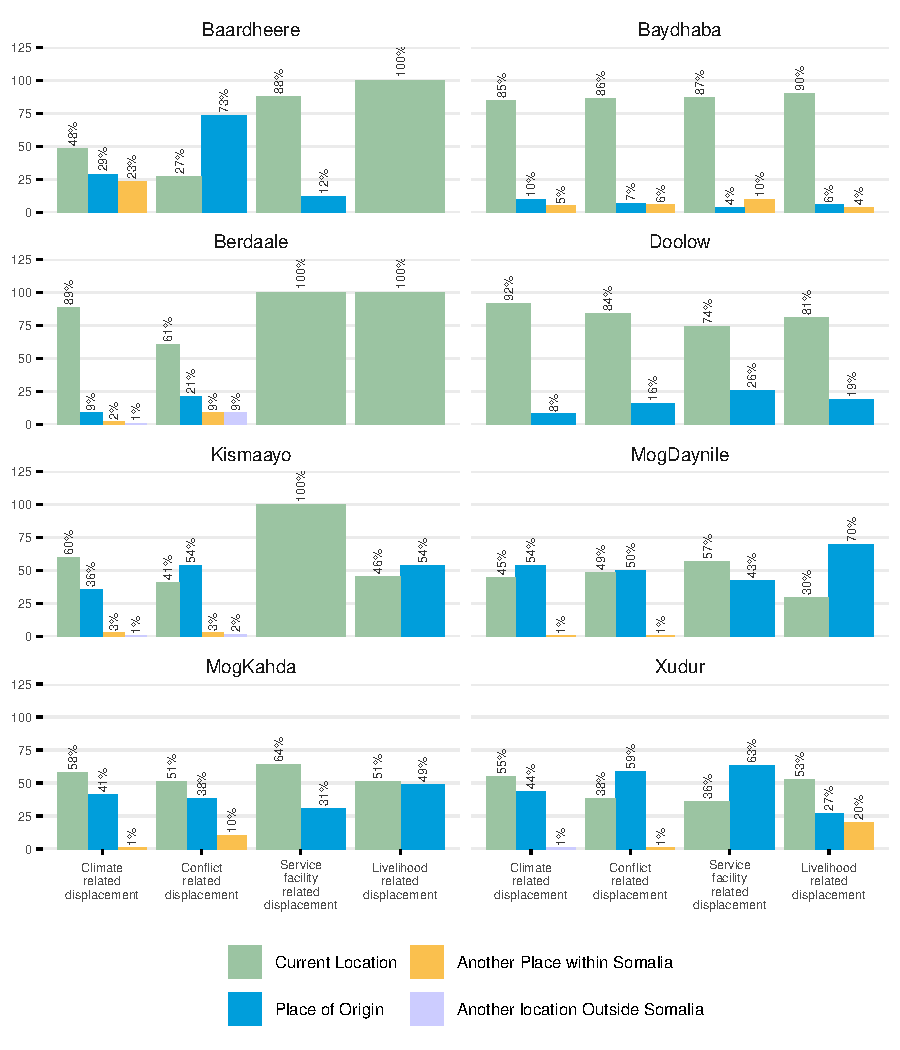
\includegraphics{climate_vs_conflict_files/figure-latex/in_classi_city-1} 

}

\caption{IDP intention vs classification by city}\label{fig:in_classi_city}
\end{figure}

\subsection{Assistance requires}\label{assistance-requires}

On average, \textbf{\emph{30\%}} of IDP households reported an intention
to return to their place of origin. However, there are notable
differences among the cities. The percentage is higher in
\emph{Mogadishu} \textbf{\emph{(53\%)}} and \emph{Xudur}
\textbf{\emph{(49\%)}}, where the number of conflict-related IDPs is
relatively greater as well \emph{(figure
\textbf{\textcolor{blue}{\ref{fig:dis_type_city}}})}.

\begin{figure}[H]

{\centering 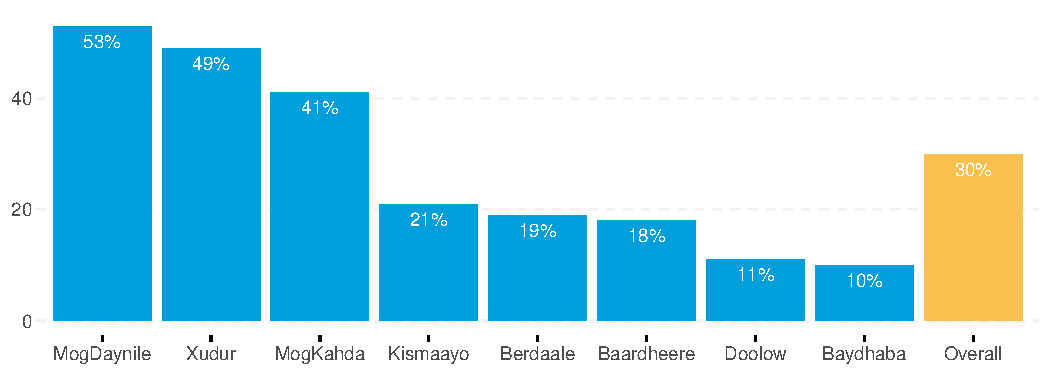
\includegraphics[width=0.8\linewidth,height=0.8\textheight]{climate_vs_conflict_files/figure-latex/unnamed-chunk-3-1} 

}

\caption{\% of IDP HH reported to have an intention to retun place of origin}\label{fig:unnamed-chunk-3}
\end{figure}

Among those who reported not intending to return to their place of
origin, many indicated they would consider returning if agricultural
support, livelihood opportunities, shelter, and basic services were made
available. However, the specific assistance required varies from city to
city. For instance, IDPs residing in \emph{Berdheree} and
\emph{Berdaale} primarily seek agricultural assistance, while residents
of \emph{Baidoa}, \emph{Kismayo}, \emph{Dollow}, and \emph{Xudur} focus
more on livelihood support. In contrast, residents of \emph{Mogadishu}
emphasize the need for basic services.

\begin{figure}[H]

{\centering 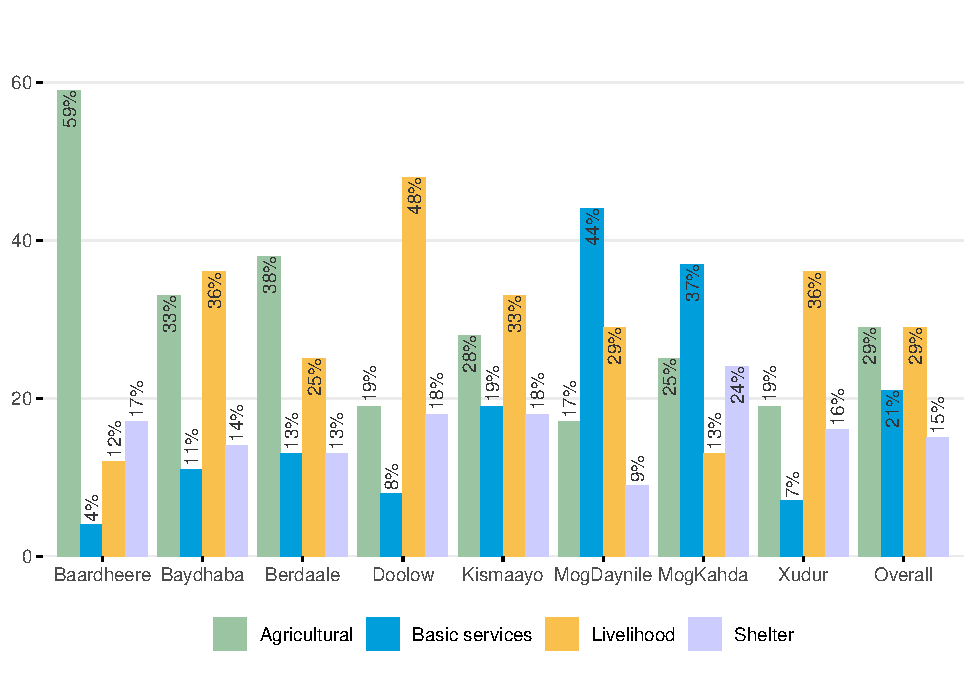
\includegraphics[width=0.8\linewidth,height=0.8\textheight]{climate_vs_conflict_files/figure-latex/unnamed-chunk-4-1} 

}

\caption{Service required}\label{fig:unnamed-chunk-4}
\end{figure}

The graph below illustrates the percentage of IDPs who do not intend to
return to their place of origin but would consider doing so if various
assistance or services were made available. \footnote{Note that the
  graph does not specify which services are needed in each city; rather,
  it reflects the perceptions of IDPs currently residing in those
  specific locations.}

\textbf{\emph{Additional Fact:}} 9\% of households reported being
displaced due to a lack of service facilities and livelihood
opportunities \emph{(figure
\textbf{\textcolor{blue}{\ref{fig:dis_type}}})}.

\subsection{Relationship between displacement month vs preferred
location be to live
long-term}\label{relationship-between-displacement-month-vs-preferred-location-be-to-live-long-term}

The DSP data indicates that in some cities, protracted IDPs are more
willing to integrate into their current location. However, this pattern
does not hold true across all cities.

\begin{figure}[H]

{\centering 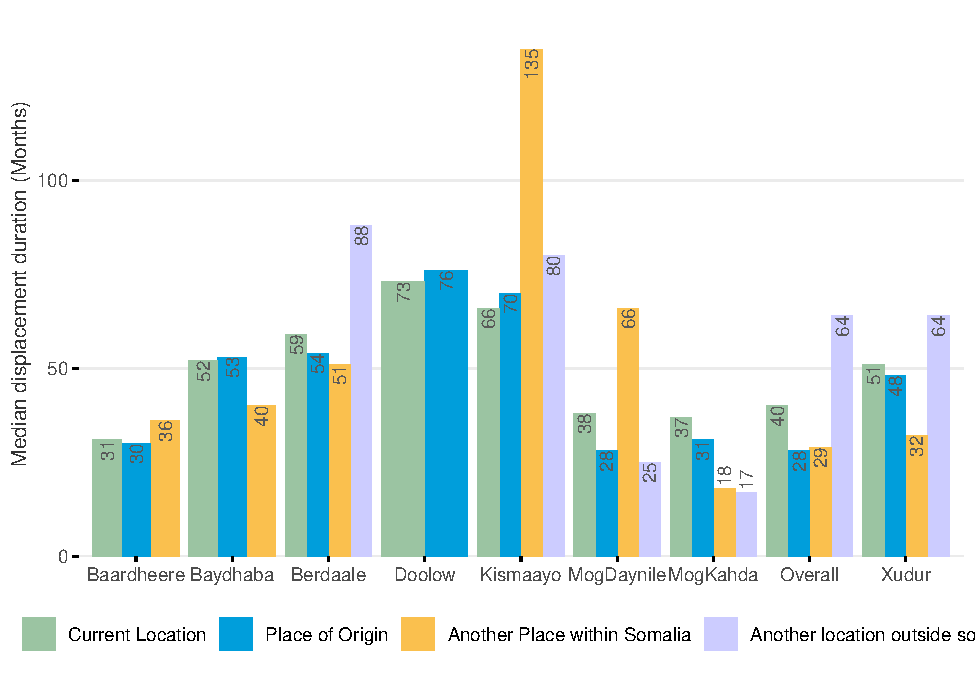
\includegraphics[width=0.8\linewidth,height=0.8\textheight]{climate_vs_conflict_files/figure-latex/unnamed-chunk-5-1} 

}

\caption{Median displacement duration by preferred location be to live long-term}\label{fig:unnamed-chunk-5}
\end{figure}

To explore any potential relationship, a weighted Chi-square test was
performed, with the following hypotheses:

\begin{itemize}
\item
  \textbf{\emph{Null hypothesis:}} Displacement duration has no effect
  on household preferences for staying in a certain location in the long
  term.
\item
  \textbf{\emph{Alternative hypothesis:}} Displacement duration does
  have an effect on household preferences for staying in a certain
  location in the long term.
\end{itemize}

The \textbf{result} indicates that the relationship between displacement
duration and long-term stay intentions varies by city, with some
locations showing a clear connection and others not. \emph{Doolow},
\emph{Kismaayo}, \emph{Baardheere}, and \emph{Baydhaba} show significant
p-values \emph{(\textless0.05)}, suggesting that displacement duration
influences long-term stay intentions in these areas. Conversely,
\emph{MogDaynile}, \emph{MogKahda}, \emph{Berdaale} and \emph{Xudur}
have p-values greater than \emph{0.05}, indicating no significant
relationship between displacement duration and the intention to stay
long-term in these cities.

\begin{longtable}[t]{lrl}
\caption{\label{tab:unnamed-chunk-7}Chi-square test between displacement duration and intention to stay long term}\\
\toprule
City & P.value & Interpretation\\
\midrule
Overall & 0.000001 & Null hypothesis is not true\\
MogKahda & 0.409740 & Null hypothesis is true\\
MogDaynile & 0.186940 & Null hypothesis is true\\
Baydhaba & 0.042260 & Null hypothesis is not true\\
Xudur & 0.999560 & Null hypothesis is true\\
\addlinespace
Doolow & 0.000010 & Null hypothesis is not true\\
Berdaale & 0.363300 & Null hypothesis is true\\
Baardheere & 0.015300 & Null hypothesis is not true\\
Kismaayo & 0.003720 & Null hypothesis is not true\\
\bottomrule
\end{longtable}

\subsection{Key findings}\label{key-findings}

\begin{itemize}
\tightlist
\item
  Climate-related displacement is the primary cause of internal
  displacement in Somalia, accounting for 74\% of cases, followed by
  conflict-related displacement at 17\%.
\item
  There is a statistically significant relationship between the reason
  for displacement and IDPs' intentions to return to their place of
  origin. Conflict-displaced IDPs are more likely to express a desire to
  return home (46\%) compared to climate-displaced IDPs (34\%).
\item
  The intention to return varies by city, with some locations showing
  different patterns. This suggests that local context plays a crucial
  role in shaping IDPs' preferences.
\item
  For IDPs not intending to return, the provision of agricultural
  support, livelihood opportunities, shelter, and basic services could
  potentially change their decision. The specific needs vary by
  location, highlighting the importance of tailored assistance programs.
\item
  The relationship between displacement duration and long-term stay
  intentions is complex and varies by city. Some locations show a clear
  connection, while others do not, indicating that protracted
  displacement doesn't uniformly lead to local integration preferences.
\end{itemize}

\end{document}
